\documentclass[10 pt]{beamer}
\usepackage{color,fancybox,bm}
\usepackage{color}
\usepackage{booktabs}
\usepackage{threeparttable}
\usepackage{dashrule}
\usepackage{float}
\usepackage{graphicx}
\usepackage{amsmath}
\usepackage{fixltx2e}
\usepackage{amssymb}
\usepackage{rotating}
\usepackage{beamerthemeshadow}
\newtheorem{acknowledgement}[theorem]{Acknowledgement}
\newtheorem{algorithm}[theorem]{Algorithm}
\newtheorem{assumption}{Assumption}
\newtheorem{assumption1}{Assumption 1}
\newtheorem{assumptions}{Assumptions}
\newtheorem{axiom}[theorem]{Axiom}
\newtheorem{case}[theorem]{Case}
\newtheorem{thm1}[theorem]{Theorem 1}
\newtheorem{thm2}[theorem]{Theorem 2}
\newtheorem{claim}[theorem]{Claim}
\newtheorem{conclusion}[theorem]{Conclusion}
\newtheorem{condition}[theorem]{Condition}
\newtheorem{conjecture}[theorem]{Conjecture}
\newtheorem{criterion}[theorem]{Criterion}
\newtheorem{exercise}[theorem]{Exercise}
\newtheorem{notation}[theorem]{Notation}
\newtheorem{proposition}[theorem]{Proposition}
\newtheorem{remark}[theorem]{Remark}
\newtheorem{summary}[theorem]{Summary}
\newcommand{\nc}{\newcommand}
\nc{\tr}{\text{tr}}

\useoutertheme{infolines}
\setbeamercolor*{palette
primary}{use=structure,fg=structure.fg,bg=structure.fg!40!white}
\setbeamercolor*{palette
secondary}{use=structure,fg=white,bg=structure.fg!60!white}
\setbeamercolor*{palette
tertiary}{use=structure,fg=white,bg=structure.fg!90!white}
\setbeamercolor*{palette quaternary}{fg=white,bg=black}

\setbeamercolor*{sidebar}{use=structure,bg=structure.fg}

\setbeamercolor*{palette sidebar
primary}{use=structure,fg=structure.fg!10} \setbeamercolor*{palette
sidebar secondary}{fg=white} \setbeamercolor*{palette sidebar
tertiary}{use=structure,fg=structure.fg!50} \setbeamercolor*{palette
sidebar quaternary}{fg=white}

\setbeamercolor*{titlelike}{use=structure,fg=structure.fg,bg=structure.fg!20!white}

\setbeamercolor*{separation line}{} \setbeamercolor*{fine separation
line}{}

\setbeamercolor*{block title example}{fg=black}

\usefonttheme[onlysmall]{structurebold}



\title[]{scRNA and Spots Data Analysis}


\author[Jinge Yu]{Jinge Yu \\[2mm]}
\institute[]{Institute of Statistics \\ Renmin University of China\\[4mm]
	
}

\date{}

\begin{document}
	
	\begin{frame}
	\titlepage
\end{frame}


\begin{frame}{Introduction}

\begin{itemize}
	\item Explore heterogeneity at celluar level.
	~\\
	~\\
	\item Cluster cells using scRNA-seq.
	~\\
	~\\
	\item Spatial organization.
	~\\
	~\\
	\item Aims at finding a cluster method detecting the heterogeneity between different spots, and cluster different cells at the same time.
\end{itemize}
\end{frame}

\begin{frame}{Data Preprocessing}
\begin{itemize}
	\item Dimensions. scRNA: $19831 \times 2000$, ST: $16528\times 996$.
	\item Data normalization(remove scale effects).
              $$  x =  x * \frac{median\{ss\}}{ss}$$
              	where $ss$ is sum of gene expression level of oen cell,  $x$ vector is the gene expresseion levels of one cell. 
	\item Continuous transformation:
           	$$x = log(2(x+1))$$
           	where x represents every single value in the data set.
	\end{itemize}
\end{frame}


\begin{frame}{Heatmap}

	We choose the most 1000 variable genes to plot maps and do data analysis, where 'the most variable' means the genes has larger  standard deviation. Notice that we chose them based on normalization data instead of original ones. Plot heatmap of two data sets:
	~\\
	~\\
	\centerline{\includegraphics[scale=0.1]{pic/heat_scrna.png}
		\includegraphics[scale=0.1]{pic/st_heat_500.png}}
	~\\
	\begin{itemize}
	\item Heatmaps revels that scRNA data is easier to cluster than spots data.
	\item Ordinary method may fail in identifying spots heterogeneity.
	\end{itemize}
\end{frame}



\begin{frame}{K-means Cluster}
Try K-means cluster on both data sets.
~\\
~\\
\centerline{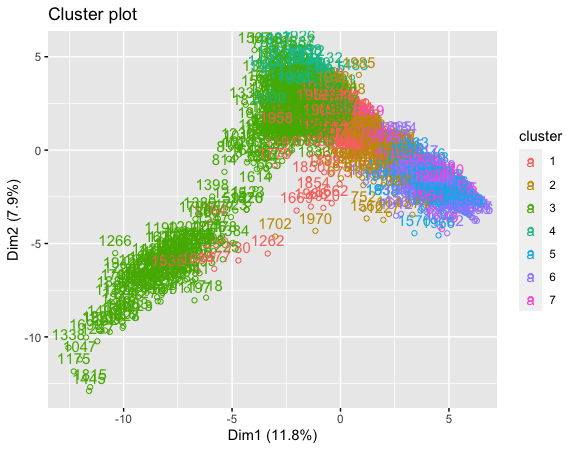
\includegraphics[scale=0.27]{pic/rna_kmeans.png}
	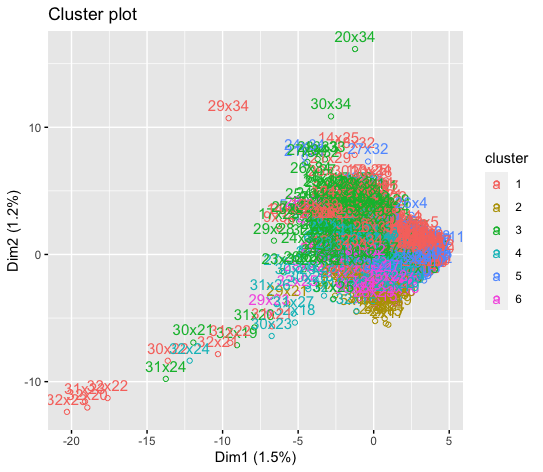
\includegraphics[scale=0.26]{pic/sp_kmeans.png}}
~\\
\begin{itemize}
	\item K-means cluster did poor in both data sets, especailly in the spots data.
	\end{itemize}
\end{frame}

\begin{frame}{Spot}
\begin{itemize}
	\item scRNA-seq can not capture spatial features of cells, since the cells are dissolved one by one.
	~\\
	~\\
	\item We use spots to explore the spatial structure of cells.
	~\\
	~\\
	\item Spot can be viewed as a tiny region of several cells close to each other.
	~\\
	~\\
	\item  The gene expression level in one spot is the sum of gene expression of all cells in the spot.
\end{itemize}
\end{frame}


\begin{frame}{Spot}
Sketch map of spots:

\centerline{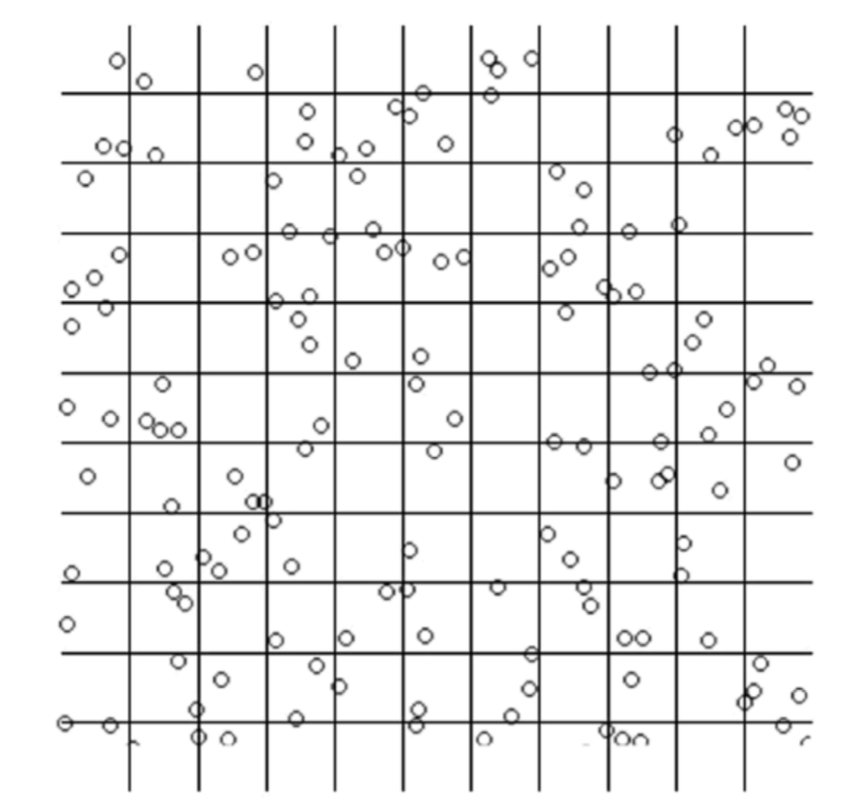
\includegraphics[scale=0.4]{pic/spot.png}}

\end{frame}

\begin{frame}{Spot}
Visualization of spots in the ST data:
\centerline{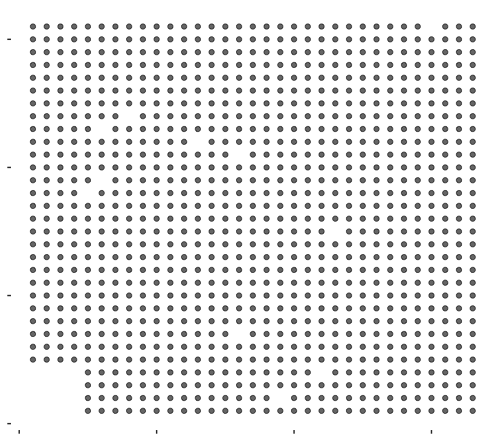
\includegraphics[scale=0.4]{pic/spots_ori.png}}

\end{frame}

\begin{frame}{Spot}
\centerline{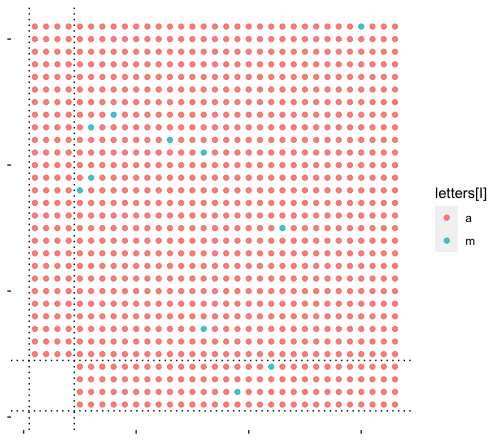
\includegraphics[scale=0.5]{pic/spots_na.png}}
\end{frame}



\begin{frame}{Null Value Spots}
There are two types of null valu spots:
\begin{itemize}
	\item Left bottom area, continuously ordered.
	\item Discretely spread.
	\end{itemize}
For the sake of calculation simplication, we fill  null value spots respectively in two ways.
\begin{itemize}
	\item Set all gene expressions levels to 0, and then transform them to continuous values.
	\item Find the neighbors of null values spots and take the average value of the neighbors.
\end{itemize}
\end{frame}

\begin{frame}{Notations}
\begin{table}
\begin{tabular}{c|c}
	\hline
	Notations & Explanation \\
	\hline
	$M$ & Number of cells \\
	\hline
	$N$ & Number of spots \\
	\hline
	$L$ & Row number of spots \\
	\hline 
	$W$ & Column number of spots \\
	\hline
	$G$ & Number of genes \\
	\hline
	$K$ & Cell types \\
	\hline 
	$S$ &Region numbers\\
	\hline
	
\end{tabular}
\end{table}
\end{frame}

\begin{frame}{Model}
As for scRNA data, we developed the following cluster method:
~\\
~\\
\begin{itemize}
	\item Model: {\tiny $$Z_{gi}|C_i = k \quad \sim\quad N(h_{gk}, \sigma^2_g).$$
	$Z_{gi}$ is the $g$-th gene expression level in cell $i$ of scRNA data\\
$C_i$ represents cell type of the $i$-th cell.}
~\\
~\\
\item Unknown parameters: \\
$C_i$,  $ h_{gk} $, $ \sigma^2_g$,$\quad i = 1,\dots M$, $g = 1,\dots,G, k = 1,\dots, K$.
~\\
~\\
\item Update $h_{gk}$, $C_i$ and $\sigma^2_g$ in turn using Bayesian method.
\end{itemize}
\end{frame}

\begin{frame}{Update parameters}
Priors:
\begin{itemize}
	\item $h_{gk} \sim N(\eta_h, \tau^2_h)$, $g = 1,\dots,G, k = 1,\dots, K$.
	\item $P(C_i = k) = \pi_{k}$, $\quad \pi_{1:K} \sim Dirichlet(\gamma_1,\dots, \gamma_1)$.
	 \item $\sigma^2_g \sim Inv-gamm(\alpha_1, \beta_1)$.
\end{itemize}
Posteriors:
\begin{itemize}
	\item $h_{gk} |- \sim N(\hat{h_{gk}}, (N_k/\sigma^2_g + 1/\eta^2_h)^{-1})$,  $g = 1,\dots,G, k = 1,\dots, K$.\\
	where $\hat{h_{gk}} = \frac{N_k\overline{Z_{gk}}/\sigma^2_g + \eta_h/\tau^2_h}{N_k/\sigma^2_g + 1/\eta^2_h}$,\\
	 $N_k = \sum_{i = 1}^M \mathbb{I}(C_i = k)$,
	$\overline{Z_{gk}} = \frac{1}{N_k}\sum_{i = 1}^M Z_{gi}\mathbb{I}(C_i = k)$.
	\item $\frac{1}{\sigma^2_g}| - \sim gamma(\frac{M}{2} + \alpha_1, \beta_1 + \frac{1}{2}\sum_{i = 1}^M (Z_{gi} - h_{c_ig})^2)$
	\item $P(C_i = k|-) = \frac{\prod_{g = 1}^G N(Z_{gi}: h_{gk}, \sigma^2_g)}{\sum_{k = 1}^K \prod_{g = 1}^G N(Z_{gi}: h_{gk}, \sigma^2_g)}$
\end{itemize}
\begin{remark}
	The notation '-' stands for given other paramters.
	\end{remark}
\end{frame}

\begin{frame}{Potts Model}
We consider potts model to obtaion spaital relations between spots.\\
Notatioins:
\begin{itemize}
	\item $(l,w)$, coordinate of a spot. We divide the spatial into a matrix of $L \times W$.
	~\\
	~\\
	\item $R_{lw}$, the region which spot $(l,w)$ belongs to. $R = R_{lw}$, $1\le l \le L$, $1\le w\le W$. $R_{lw} \in \{1,2,..., S\}$
	~\\
	~\\
	\item $\Theta = (\theta{ss^{\prime}})$, interaction energy matrix, whose diagnoal element are zero.
	~\\
	~\\
	\item $X = \{x_{lwg]}: 1\le l \le L,\quad 1\le w \le W,\quad 1\le g \le G  \}$, observed spots data.
	\end{itemize}

\end{frame}

\begin{frame}
Models:
\begin{itemize}
	\item $x_{lwg} | R_{lw} = s  \sim N(\mu_{sg}, \sigma^{\prime 2}_g) $.
	\item $Pr(R|\Theta) = \frac{1}{C(\Theta)}exp\{-H(R|\Theta)\}$.
	\item $H(R|\Theta) = -\sum_{(l,w)\sim(l^{\prime},w^{\prime})}\theta_{R_{lw}R_{l^{\prime}w^{\prime}}} \mathbb{I}(R_{lw} \neq R_{l^{\prime}w^{\prime}})$
	\item $H(R_{lw}|R_{-l,-w},\Theta) = -\sum_{(l^{\prime},w^{\prime})\in Nei(l,w)}\theta_{R_{lw}R_{l^{\prime}w^{\prime}}} \mathbb{I}(R_{lw} \neq R_{l^{\prime}w^{\prime}})$
\end{itemize}
~\\
Priors:
\begin{itemize}
\item $\theta{ss^{\prime}} \sim N(\eta_{\theta}, \tau_{\theta}^2)\quad$

\item $\mu_{sg} \sim N(\eta_{\mu}, \tau_{\mu}^2)$

\item $\sigma_g^{\prime 2} \sim $Inv-gamma$(\alpha_2,\beta_2)$
\end{itemize}
~\\
Update parameters by Gibbs sampling:
\begin{itemize}
	\item $\mu_{sg}(1\le s \le S, \quad 1\le g \le G)$
	\item $\sigma_g^2(1\le g \le G)$
	\item $R_{lw} (1\le s \le S, \quad 1\le w \le W)$,
	\item $\Theta = (\theta{ss^{\prime}}),\quad  (1\le s \le S, \quad 1\le s^{\prime} \le S,\quad s \neq s^{\prime})\quad$
\end{itemize}
\end{frame}

\begin{frame}{Double MH }
 Intractable normalizing constant $C(\Theta)$ in the posterior distributioin of $\theta_{ss^{\prime}}$. \\
 We consider Double Metropolis–Hastings algorithm to sample $\theta_{ss^{\prime}}$. \\
 The DMH algorithm iterates between the following steps:
 ~\\
 ~\\
 \begin{itemize}
 	\item Sample $\theta_{ss^{\prime}}^{\star}$ from prposal distribution $N(\theta_{ss^{\prime}}, \tau_0^2)$.
 	\item Simulate auxiliary variable $y\sim \mathbb{P}_{\Theta^{\star}}(y|R)$.
 	\item Calculate the MH ratio:
 	$$ r = \frac{N(\theta_{ss^{\prime}}^{\star};\eta_{\theta}, \tau_{\theta}^2)N(\theta_{ss^{\prime}};\theta_{ss^{\prime}}^{\star},\tau_0^2)\mathbb{P}(R|\Theta^{\star})\mathbb{P}(y|\Theta)}{N(\theta_{ss^{\prime}};\eta_{\theta},\tau_{\theta}^2)N(\theta_{ss^{\prime}}^{\star};\theta_{ss^{\prime}},\tau_0^2)\mathbb{P}(R|\Theta)\mathbb{P}(y|\Theta^{\star})}$$
 	\item Accept $\theta_{ss^{\prime}}^{\star}$ with probability $\min \{ 1,r \}$.
 	\end{itemize}
\end{frame}

\begin{frame}{Results}
We use BIC to define the best cluster number of both models.
As for scRNA model:
~\\
~\\
\centerline{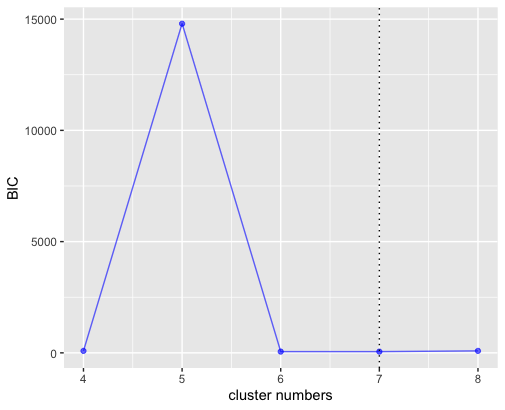
\includegraphics[scale=0.3]{pic/BIC_sc.png}}

\begin{table}
	\begin{tabular}{c|c|c|c|c|c}
		\hline
		Clusters & 4 & 5& 6& 7 & 8  \\
		\hline
		BIC value & 87.88 & 14794.44 & 56.19 & 55.55& 88.09 \\
		\hline
		
	\end{tabular}
\end{table}
So that 7 is the best cluster number.
\end{frame}

\begin{frame}{Cluster result}
I used umap method to perform dimension reduction on genes, and the result is as follows:
~\\
\centerline{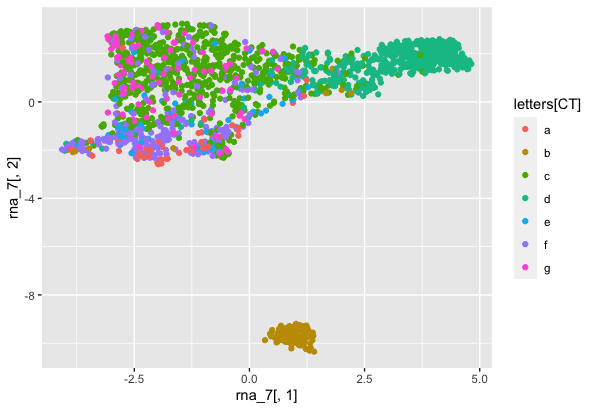
\includegraphics[scale=0.4]{pic/umap.png}}
\begin{table}
	\begin{tabular}{c|c|c|c|c|c|c|c}
		\hline
Cluster index &1&2  & 3  & 4 &  5  & 6 &  7 \\
\hline
 Number of cells& 48& 152& 796 &548 & 90 &268&  98 \\
		\hline
		
	\end{tabular}
\end{table}
\end{frame}

\begin{frame}{Iteration of parameters}
\centerline{
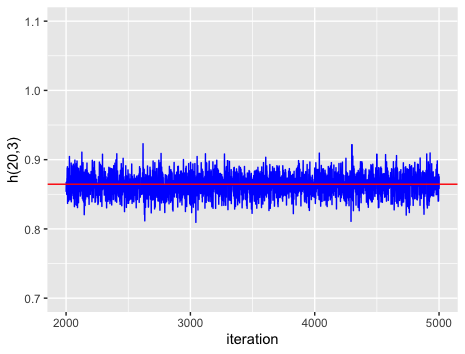
\includegraphics[scale=0.35]{pic/h_20_3_iter.png}
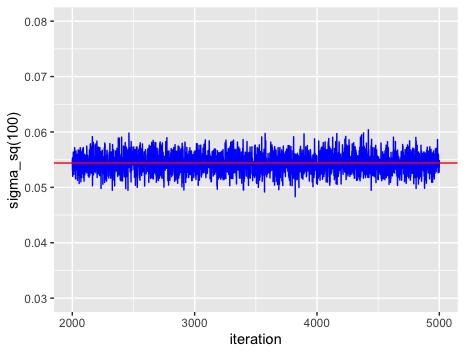
\includegraphics[scale=0.35]{pic/sgm_sq_100_iter.png}}
\end{frame}

\begin{frame}{Results}
We use BIC to define the best cluster number of both models.
As for spots model:
~\\
~\\
\centerline{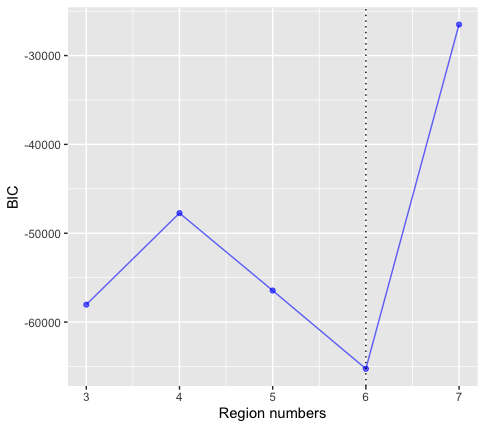
\includegraphics[scale=0.4]{pic/sp_BIC.png}}


So that 6 is the best cluster number.
\end{frame}

\begin{frame}{Cluster result}
The result is as follows:
~\\
\centerline{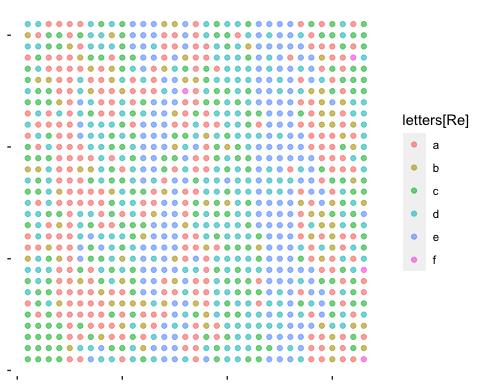
\includegraphics[scale=0.4]{pic/spk6.png}}

\end{frame}

\begin{frame}{Iteration of parameters}
\centerline{
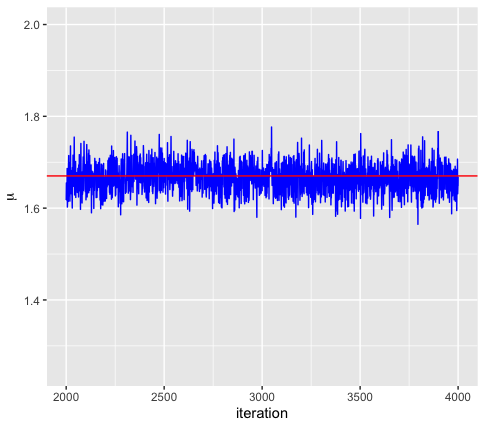
\includegraphics[scale=0.35]{pic/sp_mu_6.png}
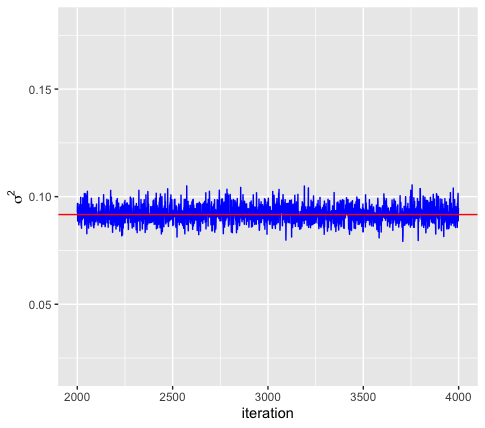
\includegraphics[scale=0.35]{pic/sp_sgm_sq_6.png}}
\end{frame}

\begin{frame}{Iteration of parameters}
\centerline{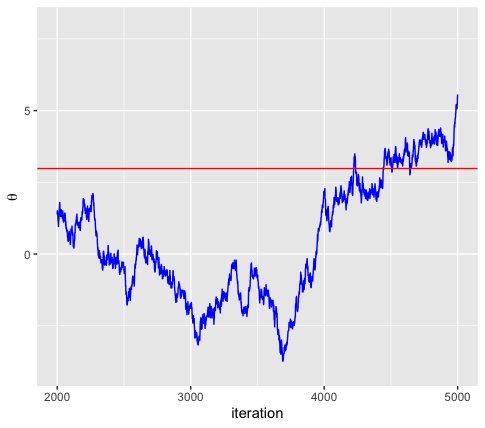
\includegraphics[scale=0.4]{pic/sp_theta_6.png}}
\begin{itemize}
	\item It seems that $\Theta$ did not reach stable state after 5000 iterations. But we cares about $R$ most, $\Theta$ is only an a auxiliary variable.
	\end{itemize}
\end{frame}

\begin{frame}{Summarize}
\begin{itemize}
	\item The two models have satisfied the demand of clustering in geeral, though the spatial one is less satisfactory.
	~\\
	~\\
	\item Take spatial orgination into consideration.
	~\\
	~\\
	\item Used Potts model and Double MH method when it comes to spatial models.
	~\\
	~\\
	\item However, every iteration took about 30-50 minutes.
\end{itemize}
\end{frame}

\begin{frame}{Future Plan}
\begin{itemize}
	\item Find a link between scRNA-seq data and spots data, integrate single-cell RNA-seq methods and microarray-based spatial models.
		~\\
	~\\
	\item Improve the speed of iteration.
		~\\
	~\\
	\item Improve the performance of spatial model.
	~\\
	~\\
	\item Figure out the deep meaning of different regions.
	\end{itemize}
\end{frame}

\end{document}